\documentclass{standalone}
\usepackage{tikz}
\usepackage{pgf-umlcd}
\usepackage{fontspec,xcolor,ifthen,xifthen,textcomp}

\setmonofont[
    AutoFakeSlant,
    BoldItalicFeatures={FakeSlant},
]{Inconsolatazi4}

\newcommand{\fieldType}[2]{\texttt{\color{red}{#1:\hspace{1mm}#2}}}
\newcommand{\funcType}[4][]{\texttt{\color{blue}{#2(#3)%
    \ifthenelse{\isempty{#4}}%
    {}%
    {\hspace{1mm}#4}%
    \ifthenelse{\isempty{#1}}%
    {}%
    {:\hspace{1mm}#1}%
}}}

\begin{document}

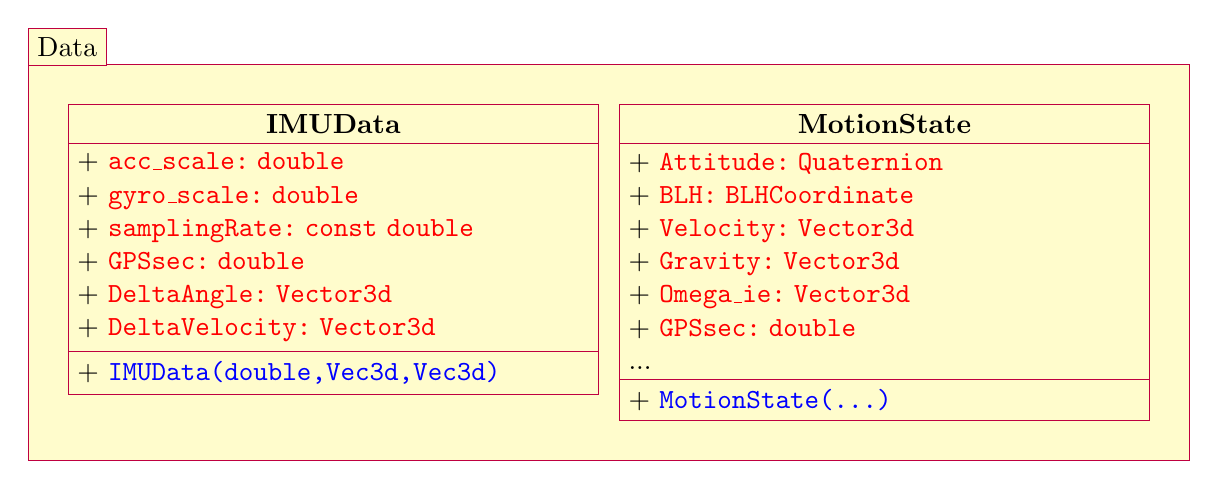
\begin{tikzpicture}
\begin{package}{Data}
\begin{class}[text width =6.5cm]{IMUData}{-3.5 , 0}
\attribute{+ \fieldType{acc\_scale}{double}}
\attribute{+ \fieldType{gyro\_scale}{double}}
\attribute{+ \fieldType{samplingRate}{const double}}
\attribute{+ \fieldType{GPSsec}{double}}
\attribute{+ \fieldType{DeltaAngle}{Vector3d}}
\attribute{+ \fieldType{DeltaVelocity}{Vector3d}}
\operation{+ \funcType{IMUData}{double,Vec3d,Vec3d}{}}
\end{class}
\begin{class}[text width =6.5 cm]{MotionState}{3.5 , 0}
    \attribute{+ \fieldType{Attitude}{Quaternion}}
    \attribute{+ \fieldType{BLH}{BLHCoordinate}}
    \attribute{+ \fieldType{Velocity}{Vector3d}}
    \attribute{+ \fieldType{Gravity}{Vector3d}}
    \attribute{+ \fieldType{Omega\_ie}{Vector3d}}
    \attribute{+ \fieldType{GPSsec}{double}}
    \attribute{...}
    \operation{+ \funcType{MotionState}{...}{}}
\end{class}
\end{package}
\end{tikzpicture}

\end{document}